Neste capítulo será apresentado em detalhes as premissas do problema de classificação visual bem como a metodologia para sua solução, que será particionada nas conforme proposto a seguir. A seção~\ref{sec:Cap3_Dataset} apresenta o conjunto de dados utilizado para o experimento.  A seção~\ref{sec:Cap3_Premissas}. apresenta as limitações e condições de contorno do problema. A seção~\ref{sec:Cap3_Proposta} apresenta a proposta de solução para o problema. A seção~\ref{sec:Cap3_Procedimentos} apresenta os procedimentos do experimento para treino e teste do modelo. Dessa forma, a metodologia será seccionada nas seguintes partes:

\begin{itemize}
    \item  Datasets.
    \item  Premissas do problema.
    \item  Proposta de solução.
    \item  Experimento para a solução do problema.

\end{itemize}

% ----------------------------------------------------------

\section{\textit{Conjunto de dados}}\label{sec:Cap3_Dataset}
Foram utilizados dois conjunto de dados, escolhidos por razões de disponibilidade e representatividade do problema. 

%% Tabelas dos datasets
%- Million A1
%ASGM Ponds Dataset https://zenodo.org/record/6400211
% Planet (URL: https://www.kaggle.com/c/planet-understanding-the-amazon-from-space/data

\subsection{Dataset amazônia do espaço}\label{sec:Cap3_Amazon_dataset}

Este dataset foi publicado em uma competição Kaggle, pela empresa Planet \footnote{https://www.kaggle.com/c/planet-understanding-the-amazon-from-space/data}. Possui resolução de 3m de pixel. Dados foram coletados dos satélites Planet Flock entre 2016 e 2017. Todas imagens são da bacia amazônica. Este dataset concerne ao desmatamento de mangues. Cada amostra é um recorde de 256x256 pixeis RGB, pertencente a 14 classes distintas. Cobrindo condições atmosféricas, coberturas de terreno e fenômenos raros. Foi utilizado em~\cite{9701667} citado no capitulo anterior.

\begin{figure}[!ht]
    \centering
    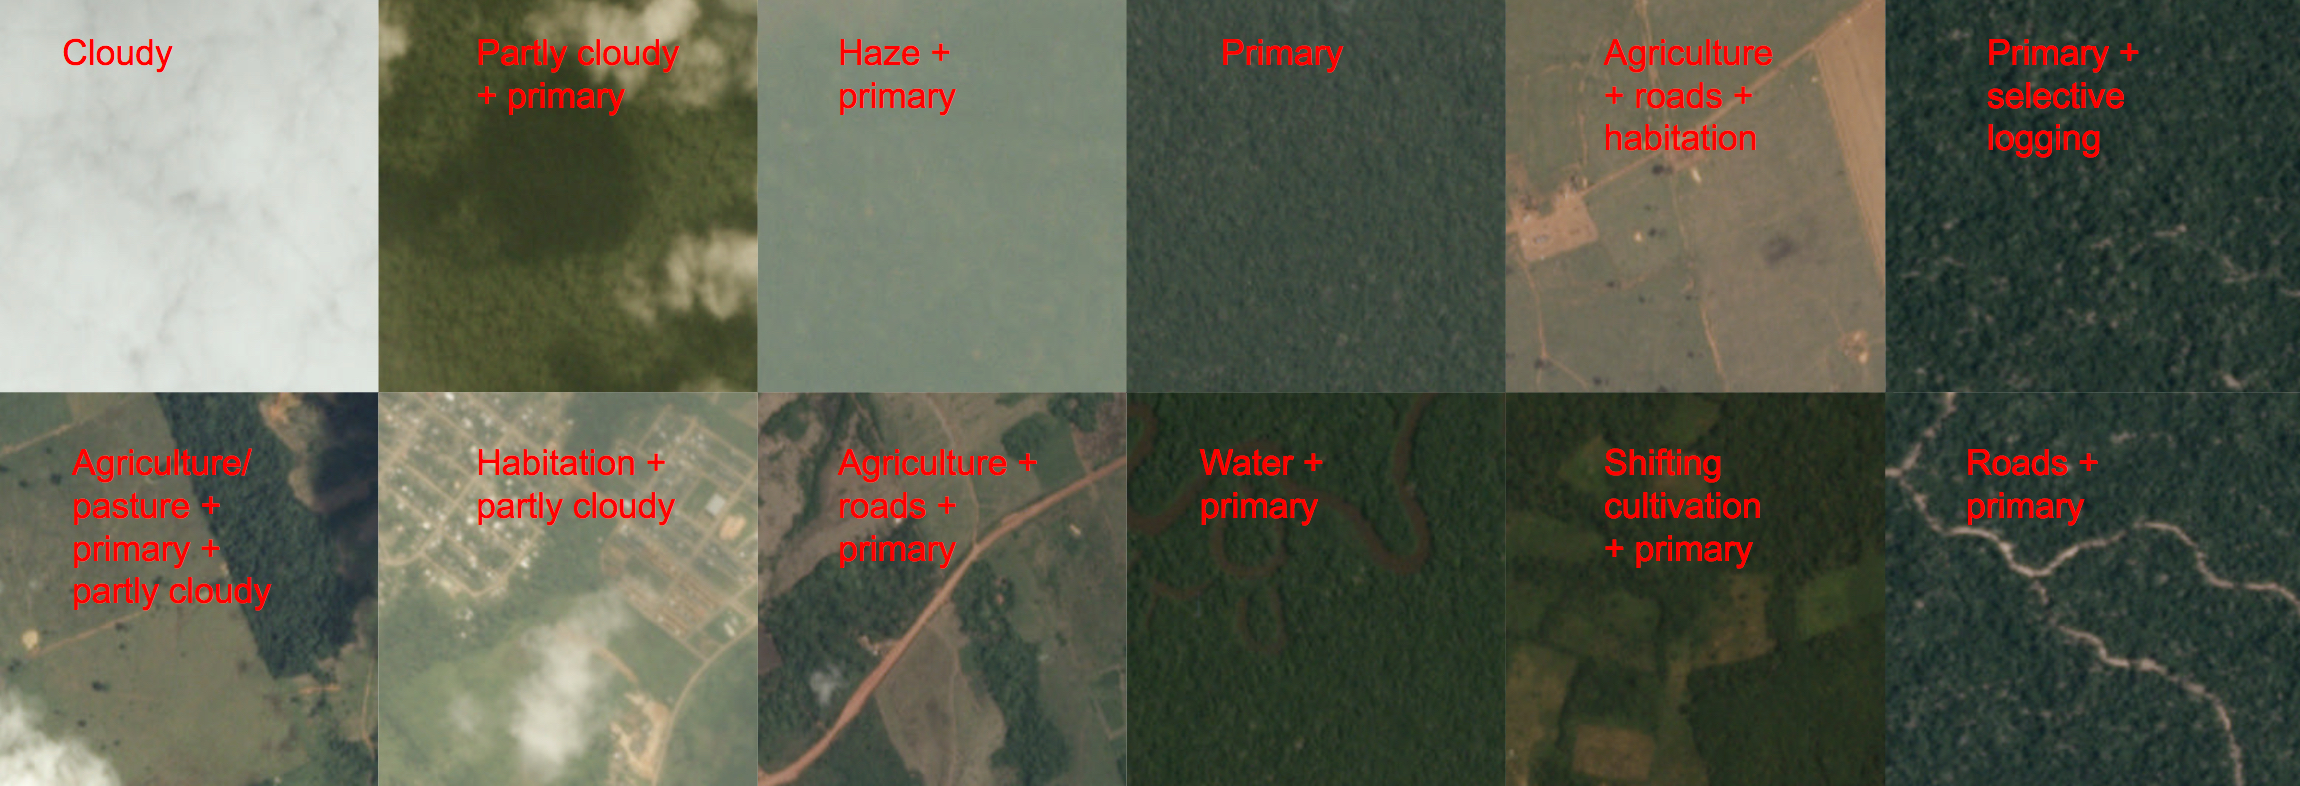
\includegraphics[width=0.9\columnwidth]{
        Imagens/chips.jpg
    }
    \caption{Amostras de classes do dataset Amazônia do espaço}
\label{fig:dataset}
\end{figure}

%We utilize a dataset (URL: https://www.kaggle.com/c/planet-understanding-the-amazon-from-space/data) published in a Kaggle competition (by Planet company), containing coarse-resolution imagery data from satellites with varying spatial resolution characteristics, i.e., the imagery has a ground-sample distance (GSD) of 3.7 m and an orthorectified pixel size of 3 m. The data comes from Planet’s Flock tow satellites in both Sun-synchronous and ISS orbits and was collected in the time interval between January 1, 2016, and February 1, 2017. All of the images are derived from the Amazon basin. Mangrove deforestation in the Amazon forest is an intense phenomenon, and a plethora of factors that contribute to deforestation is observed there. Each entry contains imagery data in RGB plus the infrared band in geo-referenced.tiff format. In our experiment, the images are classified into 14 classes and the labels are broken into three groups: atmospheric conditions, common land cover/land use phenomena, and rare land cover/land use phenomena (see Fig. 3). Here, each entry is assigned to one or more classes.


\subsection{Dataset poças de garimpo}\label{sec:Cap2_amazonia_garimpo}

Este \textit{dataset} foi utilizado em \cite{rs14071746}, mencionado no capitulo anterior. Concerne a tarefa de identificação de mudanças de imagem. Aplicadas a identificação de garimpo artesanal de ouro de pequena escala; Pode ser desafiador de se identificar, dado a variabilidade de condições atmosféricas e baixa resolução. Foram utilizadas imagens de Madre de Dios, região do Peru. Bem como amostras de outros países: Venezuela, Indonésia e Myanmar. 

% (Verificar se esse dataset é utilizável para tarefa de classificação; Resolução parece muito baixa e área muito grande)

% Abstract: Monitoring changes within the land surface and open water bodies is critical for natural resource management, conservation, and environmental policy. While the use of satellite imagery for these purposes is common, fine-scale change detection can be a technical challenge. Difficulties arise from variable atmospheric conditions and the problem of assigning pixels to individual objects. We examined the degree to which two machine learning approaches can better characterize change detection in the context of a current conservation challenge, artisanal small-scale gold mining (ASGM). We obtained Sentinel-2 imagery and consulted with domain experts to construct an open-source labeled land-cover change dataset. The focus of this dataset is the Madre de Dios (MDD) region in Peru, a hotspot of ASGM activity. We also generated datasets of active ASGM areas in other countries (Venezuela, Indonesia, and Myanmar) for out-of-sample testing.


% Dataset Description

%- Understanding the Amazon from Space [20] — multilabel dataset to track the human footprint in the Amazon rainforest; we’ll mostly refer to this as the Amazon dataset.
%WiDS Datathon 2019 [21] — binary dataset for oil palm plantation detection in Borneo; we’ll mostly refer to this as the oil palm dataset.
% Towards Detecting Deforestation [22] — binary dataset for detecting coffee plantations in the Amazon rainforest; we’ll mostly refer to this as the coffee dataset.


% ----------------------------------------------------------

\section{\textit{Premissas}}\label{sec:Cap3_Premissas}

Temos que o problema de identificação em sensoriamento remoto impõe a dificuldade de alta similaridade extra-classes e divergências intra-classes, da qual surge uma dificuldade de generalização e de viés indutivo para identificação de amostras fora das classes treinadas. Temos ainda que o treinamento de tais modelos envolvem um volume massivo de amostras e de custo computacional. 


% ----------------------------------------------------------

\section{\textit{Proposta de solução}}\label{sec:Cap3_Proposta}

Como solução para o problema, foi proposta a utilização de um modelo ViT pré-treinado com um dataset expressivo e realizar o fine-tune para o conjunto de dados de interesse. Dessa forma, obtendo um modelo com boa capacidade de generalização e com menor custo computacional para ser treinado.

Para solucionar o problema de generalização e dataset limitado da região de interesse, propomos a utilização de um modelo pré-treinado explicado em~\ref{sec:Cap2_transfer} um dataset extensivo de imagens aéreas e de satélites, de forma a aproveitar seu extrator de características, como é realizado em~\cite{wang2022empirical}. Assim o modelo será re-treinado (\textit{fine tunning}) para a região de interesse mantendo os pesos das camadas de encoder otimizar apenas a camada MLP fortemente conectadas, assim como a camadas de saída softmax. 

Dessa forma, a arquitetura proposta é o ViT apresentado em~\cite{wang2022empirical}
composta por camadas hierarquicas de encoders transformers  que funciona como extrator de características. As camadas seguintes são camadas totalmente conectadas seguidas por uma camada \textit{softmax} que realiza a classificação.
% ----------------------------------------------------------

\section{\textit{Ambiente e ferramentas}}\label{sec:Cap3_Ferramentas}


O Ambiente dos experimentos será em cadernos \textit{Jupyters}, para ser facilmente replicável e ser executável em nuvem, com a possibilidade de alugar recursos computacionais no Google Collab. Também será utilizado o \textit{framework PyTorch}, por razões de disponibilidade de métodos e conhecimentos do autor.

\subsection{\textit{PyTorch}}\label{sec:Cap2_PyTorch}
Pytorch é um \textit{framework}\footnote{Ferramental} código aberto de Python para aprendizado de máquinas. É implementado em linguagens C++ e CUDA para otimizações de computações numéricas e matriciais, que são extensivas para esta aplicação.
Foi desenvolvido pelo Facebook e é atualmente amplamente adotado pela comunidade de pesquisa e mercado de aprendizado de máquina. Possui muitas implementações das ferramentas mais utilizadas, especificamente aplicadas a \textit{Deep Learning} e visão computacional. Tem ampla adoção devido à intenção de ser um \textit{framework} de fácil uso e alto nível, com muitas abstrações e técnicas já implementadas.


% ----------------------------------------------------------


% TODO: citar o paper de aplicação direta
\section{\textit{Experimentos}}\label{sec:Cap3_Experimentos}

Para a construção da nossa solução desejada, experimentaremos combinar um modelo pré-treinado com camadas internas e de saída treinadas para a região de interesse.
Consiste em fazer experimentos em uma complexidade crescente, e replicando resultados para garantir corretude. Será simplificado a reprodução para apenas um \textit{dataset}.


Para obter o modelo proposto e de melhor desempenho, foi proposto a seguinte sequência de experimentos para construir o modelo final:

\begin{enumerate}
\item  Replicar experimentos dos trabalhos \ref{sec:Cap2_million} com \textit{checkpoints} \footnote{Captura dos pesos de uma rede a partir de certo ponto do processo de treino} disponibilizados. 
\item  Replicar experimentos de \ref{sec:Cap2_ForestViT} em um modelo base de comparação baseado em em uma CNN ResNet-50
\item  Replicar o experimento do \ref{sec:Cap2_ForestViT} utilizando um modelo ViT pré treinado para sensoriamento remoto
\item Avaliar desempenho, comparar com os experimentos e trabalhos bases\ref{sec:Cap2_revisao_literatura}
\end{enumerate}


    
% ----------------------------------------------------------

\section{\textit{Procedimentos}}\label{sec:Cap3_Procedimentos}

Os procedimentos do experimento principal consiste principalmente nas etapas de 
pré-processamento, treino e validação. Explicadas a diante.

\subsection{\textit{Pré-processamento}}\label{sec:Cap3_PreProcess}
O pré-processamento consistem em preparar as amostras do conjunto de dados de interesse para treino e validação. Para o conjunto de dados floresta amazônica temos 40000 amostras de treino e 4000 de teste. Cada recorte de resolução 256x256 px é aplicado um \textit{downsampling}\footnote{subamostragem} para a resolução de entrada do modelo pré-treinado, de 224 × 224. 

\subsection{\textit{Treino}}\label{sec:Cap3_Treino}
Para a etapa de treino, utilizamos a arquitetura proposta em~\ref{sec:Cap3_Proposta}, que consiste de um modelo pré-treinado, e retreinando suas ultimas camadas de classificação por camadas fortemente conectadas seguidas de camadas de \textit{softmax}, como ilustra a imagem a seguir:


TODO Imagem da arquitetura proposta.



\subsection{\textit{Validação}}\label{sec:Cap3_Validacao}

A etapa de validação será realizada a medida do desempenho do modelo no conjunto de testes para classificação.




% Chip (Image) Data Format

% The chips for this competition were derived from Planet's full-frame analytic scene products using our 4-band satellites in sun-synchronous orbit (SSO) and International Space Station (ISS) orbit. The set of chips for this competition use the GeoTiff format and each contain four bands of data: red, green, blue, and near infrared. The specific spectral response of the satellites can be found in the Planet documentation. Each of these channels is in 16-bit digital number format, and meets the specification of the Planet four band analytic ortho scene product.

% For purposes of the competition we have stripped out all of the geotiff information regarding the chip footprint and ground control points (GCPs). The imagery has a ground-sample distance (GSD) of 3.7m and an orthorectified pixel size of 3m. The data comes from Planet's Flock 2 satellites in both sun-synchronous and ISS orbits and was collected between January 1, 2016 and February 1, 2017. All of the scenes come from the Amazon basin which includes Brazil, Peru, Uruguay, Colombia, Venezuela, Guyana, Bolivia, and Ecuador (see map below).

% We have also included a set of JPG chips for reference and practice. These chips were processed using the Planet visual product processor and then saved as jpg chips. These chips are provided as a reference to the scene content, but we expect that the additional information in the tif chips will be more fruitful for the competition.

% https://commons.wikimedia.org/w/index.php?curid=4745680 Above: A map of the Amazon basin.
% Labeling Process and Data Quality

% enter image description here

% To assemble this data set we set out with an initial specification of the phenomena we wished to find and include in the final data set. From that initial specification we created a "wish list" of scenes where we included a ballpark number of scenes required to get a sufficient number of chips to demonstrate the phenomena. This initial set of scenes was painstakingly collected by our Berlin team using Planet Explorer. All told this initial set of scenes numbered approximately 1600 and covered a land area of thirty million hectares.

% This initial set of scenes was then processed using a custom product processor to create the jpg and 4-band tif chips. Any chip that did not have a full and complete four band product was omitted. This initial set of over 150,000 chips was then divided into two sets, a "hard" and an "easy" set. The easy set contained scenes that the Berlin team identified as having easier-to-identify labels like primary rainforest, agriculture, habitation, roads, water, and cloud conditions. The harder set of data was derived from scenes where the Berlin team had selected for shifting cultivation, slash and burn agriculture, blow down, mining, and other phenomenon.

% The chips were labeled using the Crowd Flower platform and a mixture of crowd-sourced labor and our Berlin and San Francisco teams. While the utmost care was taken to get a large and well-labeled dataset, we are aware that not all of the labels in our dataset are correct. Governments around the world retain a large number of highly trained analysts to review images and even they can't always agree on what is present in a given satellite image.

% Moreover, the commonly prescribed approach for labeling data in the GIS community is to use actual ground truth data to label scenes, which is both costly and time consuming. With this in mind we do believe our data has a reasonably high signal to noise ratio and is sufficient for training. Given the ease and expediency of crowd labeling, we believe that a large, relatively inexpensive and rapidly labeled dataset is better than a small, more definitive but less diverse dataset. We are interested to see how competitors handle any inaccuracies.
% Class Labels

% The class labels for this task were chosen in collaboration with Planet's Impact team and represent a reasonable subset of phenomena of interest in the Amazon basin. The labels can broadly be broken into three groups: atmospheric conditions, common land cover/land use phenomena, and rare land cover/land use phenomena. Each chip will have one and potentially more than one atmospheric label and zero or more common and rare labels. Chips that are labeled as cloudy should have no other labels, but there may be labeling errors. Sample chips with labels

% Above: Sample chips and their labels.

% As discussed in the data collection portion of this document, the chip labels are inherently noisy due to the labeling process and ambiguity of features, and scenes may either omit class labels or have incorrect class labels. Part of the challenge of this competition is to figure out how to work with noisy data.
% Cloud Cover Labels

% Clouds are a major challenge for passive satellite imaging, and daily cloud cover and rain showers in the Amazon basin can significantly complicate monitoring in the area. For this reason we have chosen to include a cloud cover label for each chip. These labels closely mirror what one would see in a local weather forecast: clear, partly cloudy, cloudy, and haze. For our purposes haze is defined as any chip where atmospheric clouds are visible but they are not so opaque as to obscure the ground. Clear scenes show no evidence of clouds, and partly cloudy scenes can show opaque cloud cover over any portion of the image. Cloudy images have 90% of the chip obscured by opaque cloud cover.
% Examples of Cloudy Scenes

% Cloudy Scene enter image description here
% Examples of Partly Cloudy Scenes

% Partly Cloudy Scene Partly Cloudy Scene
% Examples of Hazy Scenes

% Partly Cloudy Scene Partly Cloudy Scene
% More Common Labels

% The common labels in this data set are rainforest, agriculture, rivers, towns/cities, and roads. Examples of each class are given below.
% Primary Rain Forest

% The overwhelming majority of the data set is labeled as "primary", which is shorthand for primary rainforest, or what is known colloquially as virgin forest. Generally speaking, the "primary" label was used for any area that exhibited dense tree cover.This Mongobay article gives a concise description of the difference between primary and secondary rainforest, but distinguishing between the two is difficult solely using satellite imagery. This is particularly true in older "secondary" forests. Primary Rainforest

% Above: Approximately 25,000 acres of untouched primary rainforest.
% Water (Rivers & Lakes)

% Rivers, reservoirs, and oxbow lakes are important features of the Amazon basin, and we used the water tag as a catch-all term for these features. Rivers in the Amazon basin often change course and serve as highways deep into the forest. The changing course of these rivers creates new habitat but can also strand endangered Amazon River Dolphins. River

% Above: A larger and slower river with significant sand bars. The brown color comes from significant silt deposits. River

% Above: A small tributary joins a larger river system. The deep brown color of the river is noticeable near the bright sand bars.
% Habitation

% The habitation class label was used for chips that appeared to contain human homes or buildings. This includes anything from dense urban centers to rural villages along the banks of rivers. Small, single-dwelling habitations are often difficult to spot but usually appear as clumps of a few pixels that are bright white. Habitation

% Above: A larger city in the Amazon basin. Habitation

% Above: A large city.
% Agriculture

% Commercial agriculture, while an important industry, is also a major driver of deforestation in the Amazon. For the purposes of this dataset, agriculture is considered to be any land cleared of trees that is being used for agriculture or range land.

% More reading on agriculture in the Amazon:

%     Sugarcane in Bolivia
%     Papaya cultivation destroying Peruvian Rainforest
%     Harvests in Rio Grande do Sul

% Agriculture 1

% Above: An agricultural area that showing the end state of "fishbone" deforestation. Agriculture 2

% Above: A newer agricultural area showing "fishbone" deforestation.
% Road

% Roads are important for transportation in the Amazon but they also serve as drivers of deforestation. In particular, "fishbone" deforestation often follows new road construction, while smaller logging roads drive selective logging operations. For our data, all types of roads are labeled with a single "road" label. Some rivers look very similar to smaller logging roads, and consequently there may be some noise in this label. Analysis of the image using the near infrared band may prove useful in disambiguating the two classes.

% More information: - Roads in the Amazon - NASA article on Fishbone Deforestation

% Road 1

% Above: classic "Fishbone" deforestation following a road. Road 2

% Above: roads snake out of a small town in the Amazon.
% Cultivation

% Shifting cultivation is a subset of agriculture that is very easy to see from space, and occurs in rural areas where individuals and families maintain farm plots for subsistence. This article by MongaBay by MongaBay gives a detailed overview of the practice. This type of agriculture is often found near smaller villages along major rivers, and at the outskirts of agricultural areas. It typically relies on non-mechanized labor, and covers relatively small areas. cultivation

% Above: A zoomed-in area showing cultivation (right side of river) cultivation

% Above: A zoomed-in area showing cultivation and some selective logging. Dark areas indicate recent slash/burn activity
% Bare Ground

% Bare ground is a catch-all term used for naturally occuring tree free areas that aren't the result of human activity. Some of these areas occur naturally in the Amazon, while others may be the result from the source scenes containing small regions of biome much similar to the pantanal or cerrado. bare ground

% Above: a naturally occuring bare area in the cerrado. bare ground

% Above: a naturally occuring bare area in the cerrado.
% Less Common Labels
% Slash and Burn

% Slash-and-burn agriculture can be considered to be a subset of the shifting cultivation label and is used for areas that demonstrate recent burn events. This is to say that the shifting cultivation patches appear to have dark brown or black areas consistent with recent burning.This NASA Earth Observatory article gives a good primer on the practice as does this wikipedia article. Above: ground view of slash and burn agriculture. By Alzenir Ferreira de Souza slash burn

% Above: A zoomed-in view of an area with shifting cultivation with evidence of a recent fire. slash burn

% Above: A zoomed-in view of an area with shifting cultivation and evidence of a recent fire.
% Selective Logging

% The selective logging label is used to cover the practice of selectively removing high value tree species from the rainforest (such as teak and mahogany). From space this appears as winding dirt roads adjacent to bare brown patches in otherwise primary rain forest. This Mongabay Article covers the details of this process. Global Forest Watch is another great resource for learning about deforestation and logging. logging

% Above: The brown lines on the right of this scene are a logging road. Note the small brown dots in the area around the road. logging

% Above: A zoomed image of logging roads and selective logging. logging

% Above: A zoomed image of logging roads and selective logging.
% Blooming

% Blooming is a natural phenomenon found in the Amazon where particular species of flowering trees bloom, fruit, and flower at the same time to maximize the chances of cross pollination. These trees are quite large and these events can be seen from space. Planet recently captured a similar event in Panama. bloom

% Above: a zoomed and contrast enhanced of a bloom event in the Amazon basin. The red arrows point to a few specific trees. The canopies of these trees can be over 30m across (~100ft).
% Conventional Mining

% There are a number of large conventional mines in the Amazon basin and the number is steadily growning. This label is used to classify large-scale legal mining operations.

% mine

% Above: A conventional mine in the Amazon.
% "Artisinal" Mining

% Artisinal mining is a catch-all term for small scale mining operations. Throughout the Amazon, especially at the foothills of the Andes, gold deposits lace the deep, clay soils. Artisanal miners, sometimes working illegally in land designated for conservation, slash through the forest and excavate deep pits near rivers. They pump a mud-water slurry into the river banks, blasting them away so that they can be processed further with mercury - which is used to separate out the gold. The denuded moonscape left behind takes centuries to recover.

%     Illegal and artisanal mines in Peru
%     Images of artisanal mining in Peru
%     MAAP Amazon Report #36
%     MAAP Amazon Report #49
%     Global Forest Watch article on Mining artisanal mine

% Above: A zoomed image of an artisanal mine in Peru. artisanal mine

% Above: A zoomed image of an artisanal mine in Peru.
% Blow Down

% Blow down, also called windthrow, is a naturally occurring phenomenon in the Amazon. Briefly, blow down events occur during microbursts where cold dry air from the Andes settles on top of warm moist air in the rainforest. The colder air punches a hole in the moist warm layer, and sinks down with incredible force and high speed (in excess of 100MPH). These high winds topple the larger rainforest trees, and the resulting open areas are visible from space. The open areas do not stay visible for along as plants in the understory rush in to take advantage of the sunlight.

%     MAAP #55: Blow Down Report in Peru Detailed
%     MAAP #54: Blow Down Report in Peru
%     National Geographic Article on Blow Down
%     Nature article on the size and frequency of blow down events. blow down

% Above: A recent blow down event in the Amazon circled in red. Note the light green of the forest understory and the pattern of tree loss.



